\section{Results and Validation} \label{sec:results}

\begin{table}[!htb]
    \caption{LLC resonant converter design parameters.}
    \label{tab:LLC_Parameters}
    \centering
    \renewcommand{\arraystretch}{1.3} % melhora visual (opcional)
    
    \begin{tabular}{cc}
        \hline
        Input Voltage ($V_{in}$)        & 600 V          \\ 
        Output Voltage ($V_{out}$)      & 900 V          \\ 
        Power ($P$)                    & 10 kW          \\
        Switching Frequency ($f_s$)     & 120 kHz        \\ 
        Q-Factor ($Q$)                & 0.5            \\ 
        Resonance Frequency ($f_r$)    & 118--122 kHz   \\ 
        $k$                           & 4, 5, 6        \\ 
        \hline
    \end{tabular}
\end{table}

For validation of the proposed methodology, an LLC converter with the parameters listed in Table~\ref{tab:LLC_Parameters} was designed using the data-driven efficiency mapping framework. The converter was then simulated in a time-domain circuit simulator to evaluate its steady-state performance, with emphasis on efficiency and waveform characteristics.

The data-driven design process identified resonant tank parameters that satisfy the design requirements while enabling operation close to the resonant frequency. In particular, the values of the resonant inductor ($L_r$) and capacitor ($C_r$) were selected to maximize efficiency under the specified conditions. The resulting design is summarized in Table~\ref{tab:AI_Parameters}, including the predicted efficiency.

\begin{table}[!htb]
    \caption{AI-optimized LLC resonant converter parameters.}
    \label{tab:AI_Parameters}
    \centering
    \renewcommand{\arraystretch}{1.3}
    \begin{tabular}{cc}
        \hline
        Resonance Frequency ($f_r$)       & 120 kHz   \\
        Resonant Tank Impedance ($Z_R$)   & 29.40 $\Omega$ \\
        $k$                               & 4         \\ 
        Resonant Inductor ($L_r$)         & 38.99 $\mu$H \\
        Resonant Capacitor ($C_r$)        & 45.11 $\mu$F \\
        Magnetizing Inductor ($L_m$)      & 15.59 $\mu$H \\
        Efficiency ($\eta$)               & 97.49\%   \\ 
        \hline
    \end{tabular}
\end{table}

The designed converter was simulated under the specified operating conditions, and the resulting waveforms were analyzed to validate the predicted performance. The key waveforms of interest include the input and output voltages and currents, as well as the switch voltages and currents, which were used to compute instantaneous power losses and overall efficiency.

\begin{figure}[!htb]
    \centering
    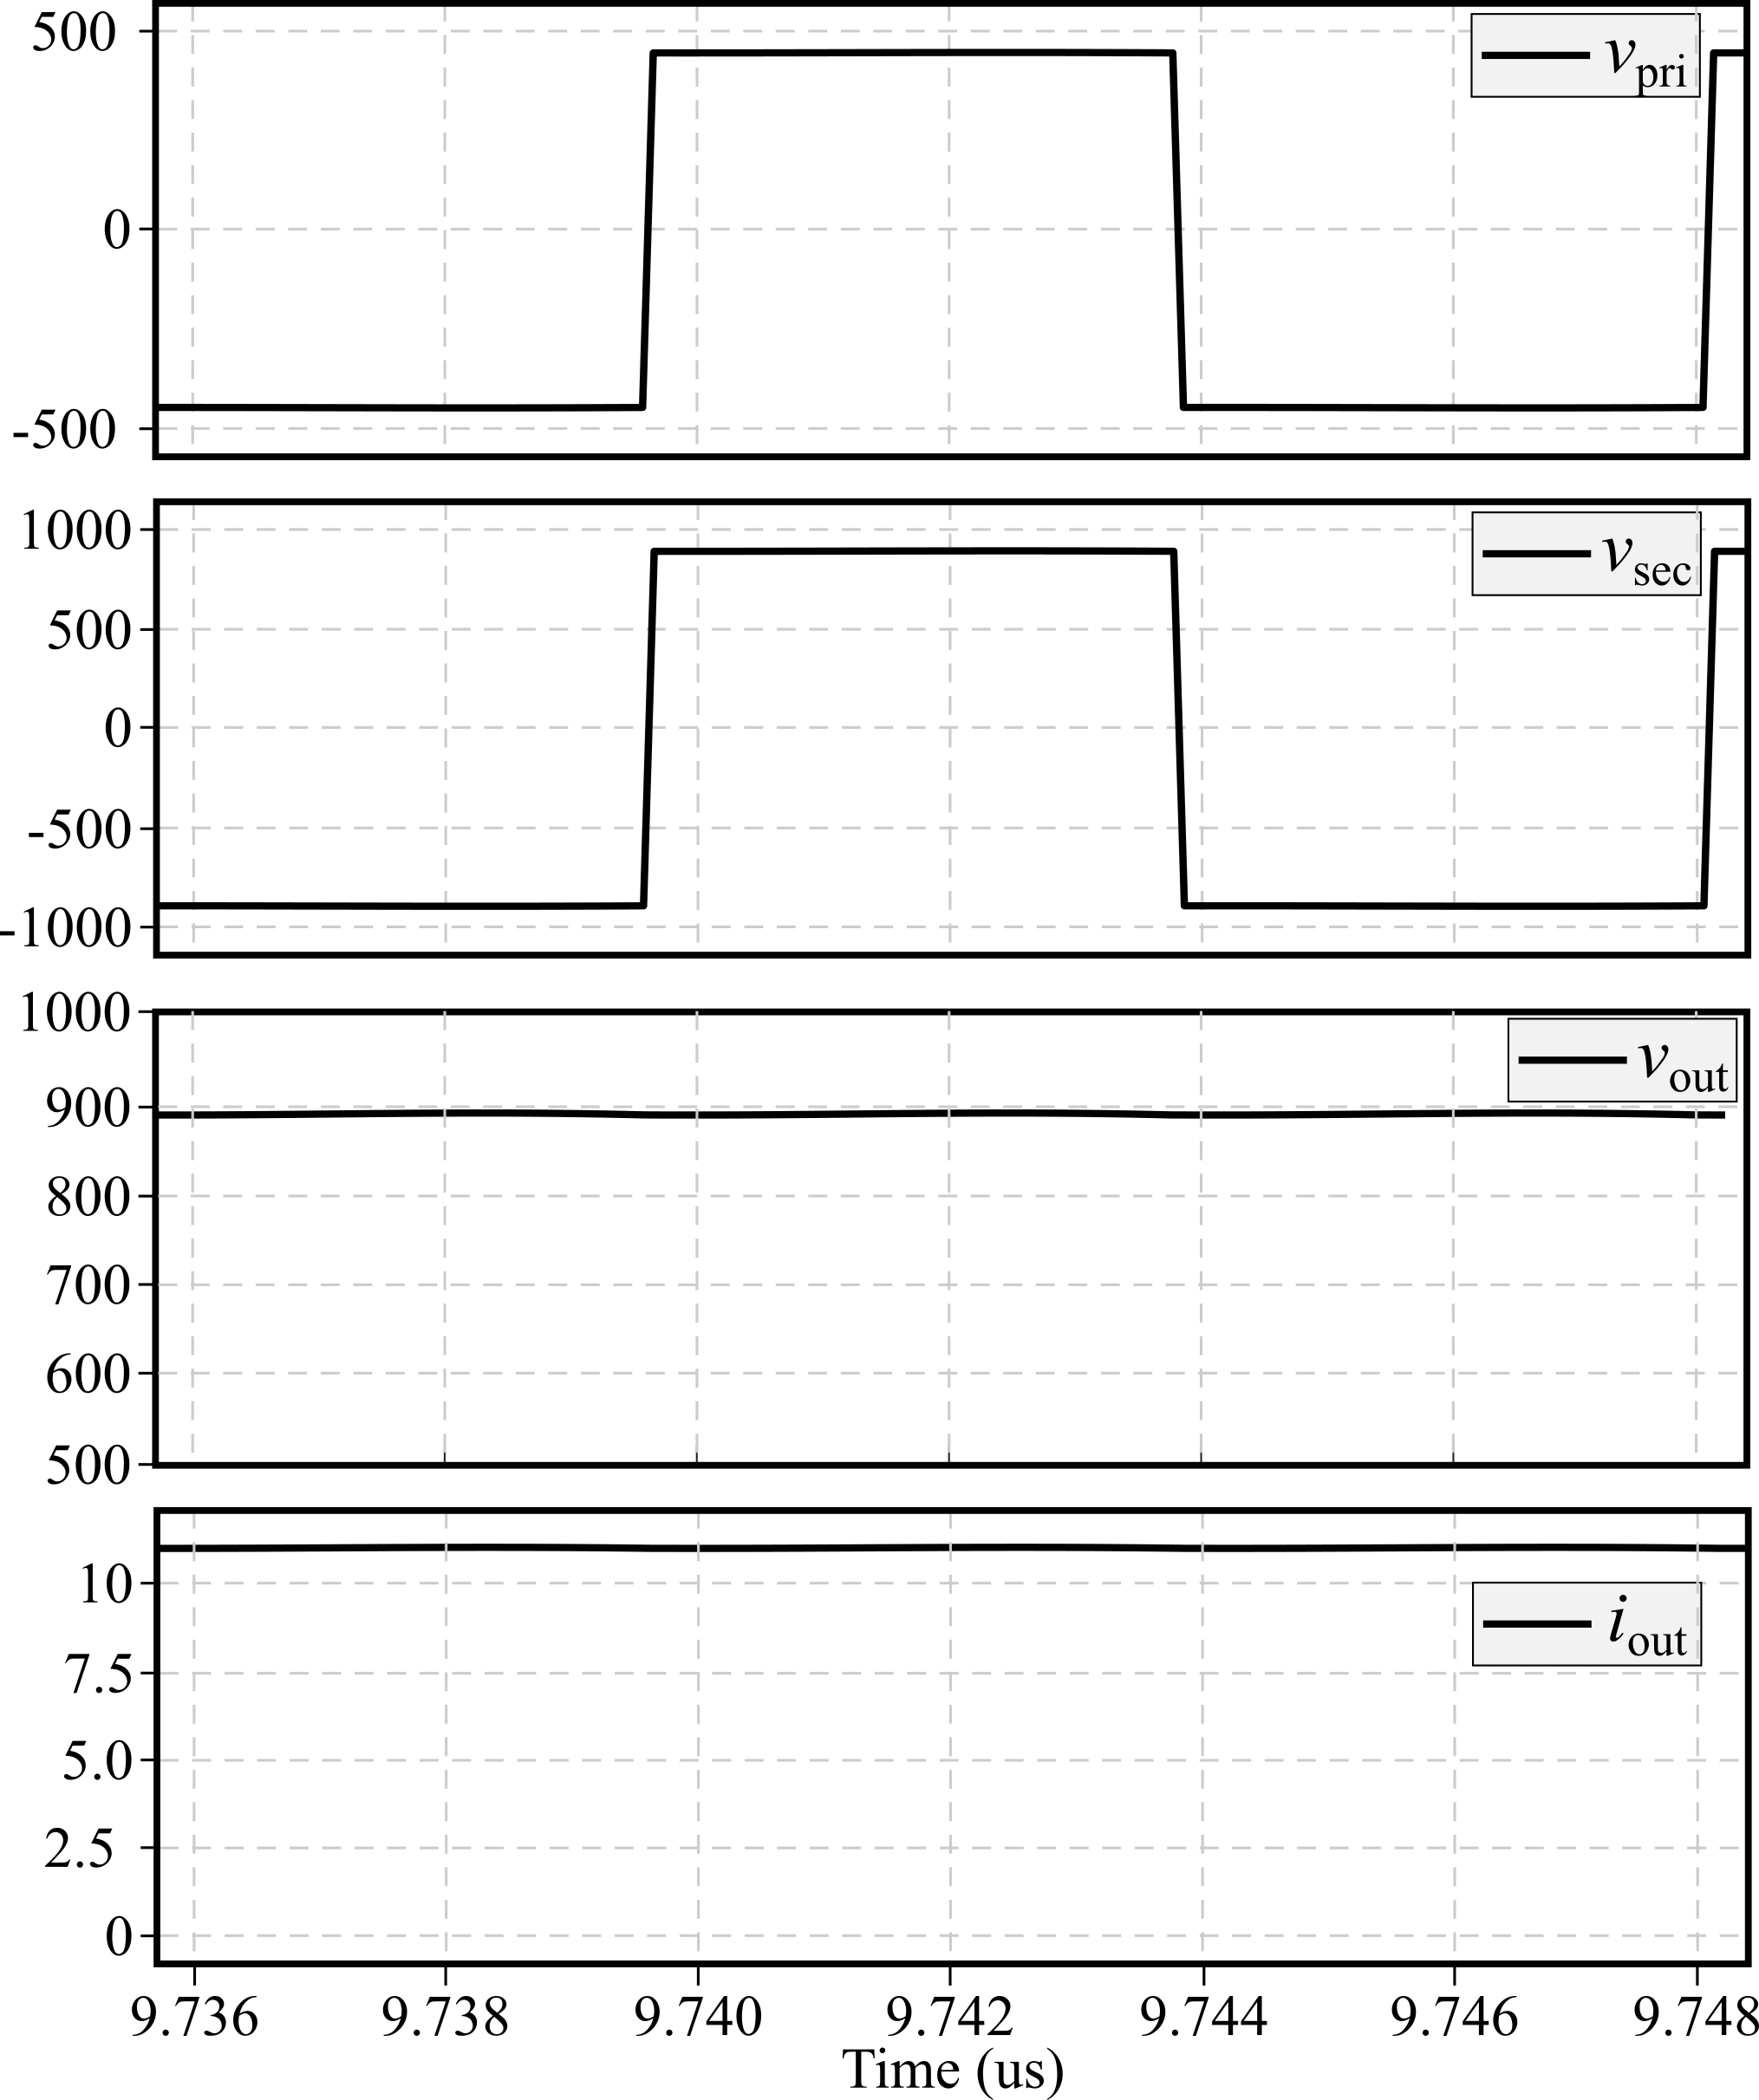
\includegraphics[width=\columnwidth]{figures/Result_1.png}
    \caption{Input and output waveforms under steady-state operation.}
    \label{fig:Result_1}
\end{figure}

Fig.~\ref{fig:Result_1} shows the simulated waveforms of the input voltage ($V_{in}$), input current ($i_{in}$), output voltage ($V_o$), and output current ($I_o$) for the designed LLC resonant converter operating at approximately 10~kW. The waveforms are obtained under steady-state conditions, with the converter operating close to the resonant frequency. The input current exhibits the pulsating behavior expected in resonant converters, reflecting the energy transfer through the resonant tank. In contrast, the output voltage and current remain nearly constant with low ripple, indicating stable operation and effective output filtering. These results confirm the correct steady-state operation of the converter under the selected operating condition.

Fig.~\ref{fig:Result_2} shows the steady-state waveforms of the input voltage ($V_{in}$), input current ($i_{in}$), inverter output voltage ($V_{AB}$), and resonant inductor current ($i_{Lr}$). The inverter output voltage $V_{AB}$ presents the expected square waveform produced by the full-bridge switching operation, while the resonant inductor current $i_{Lr}$ is nearly sinusoidal. This behavior confirms operation close to the resonant frequency and validates the expected resonant tank operation and energy transfer characteristics of the converter.

\begin{figure}[!htb]
    \centering
    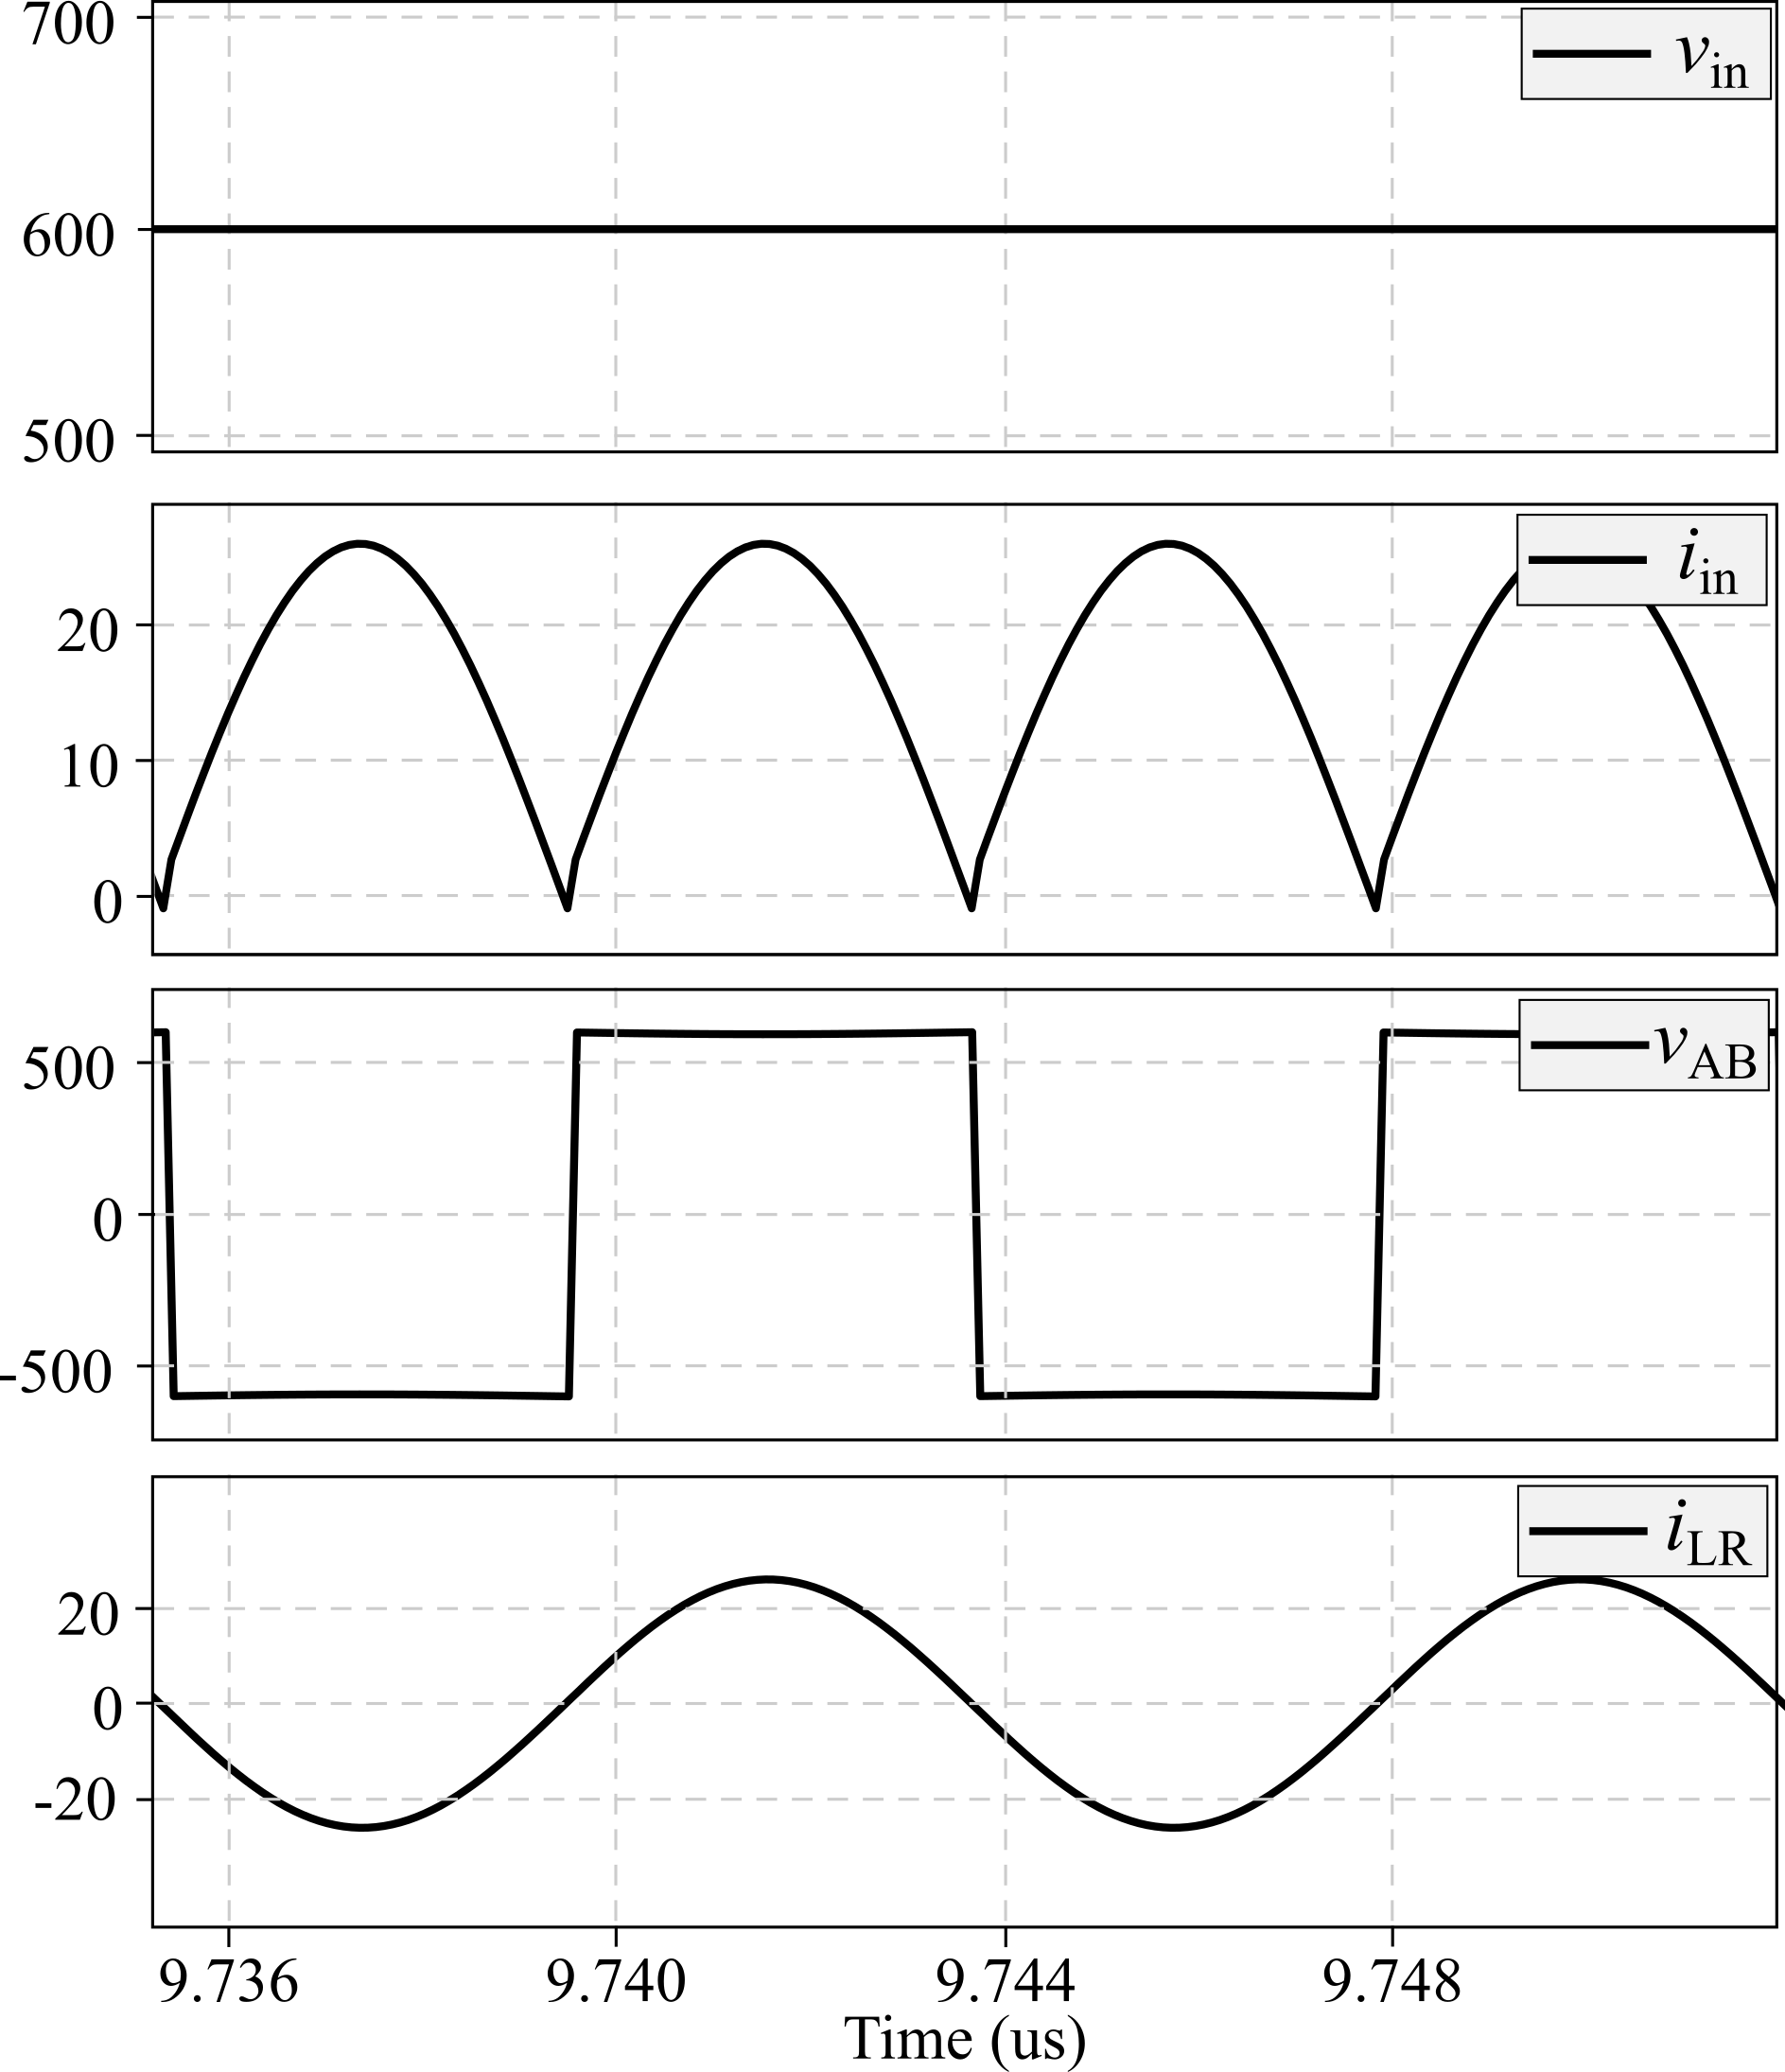
\includegraphics[width=.95\columnwidth]{figures/Result_2.png}
    \caption{Resonant tank and inverter waveforms.}    
    \label{fig:Result_2}
\end{figure}

\begin{figure}[!htb]
    \centering
    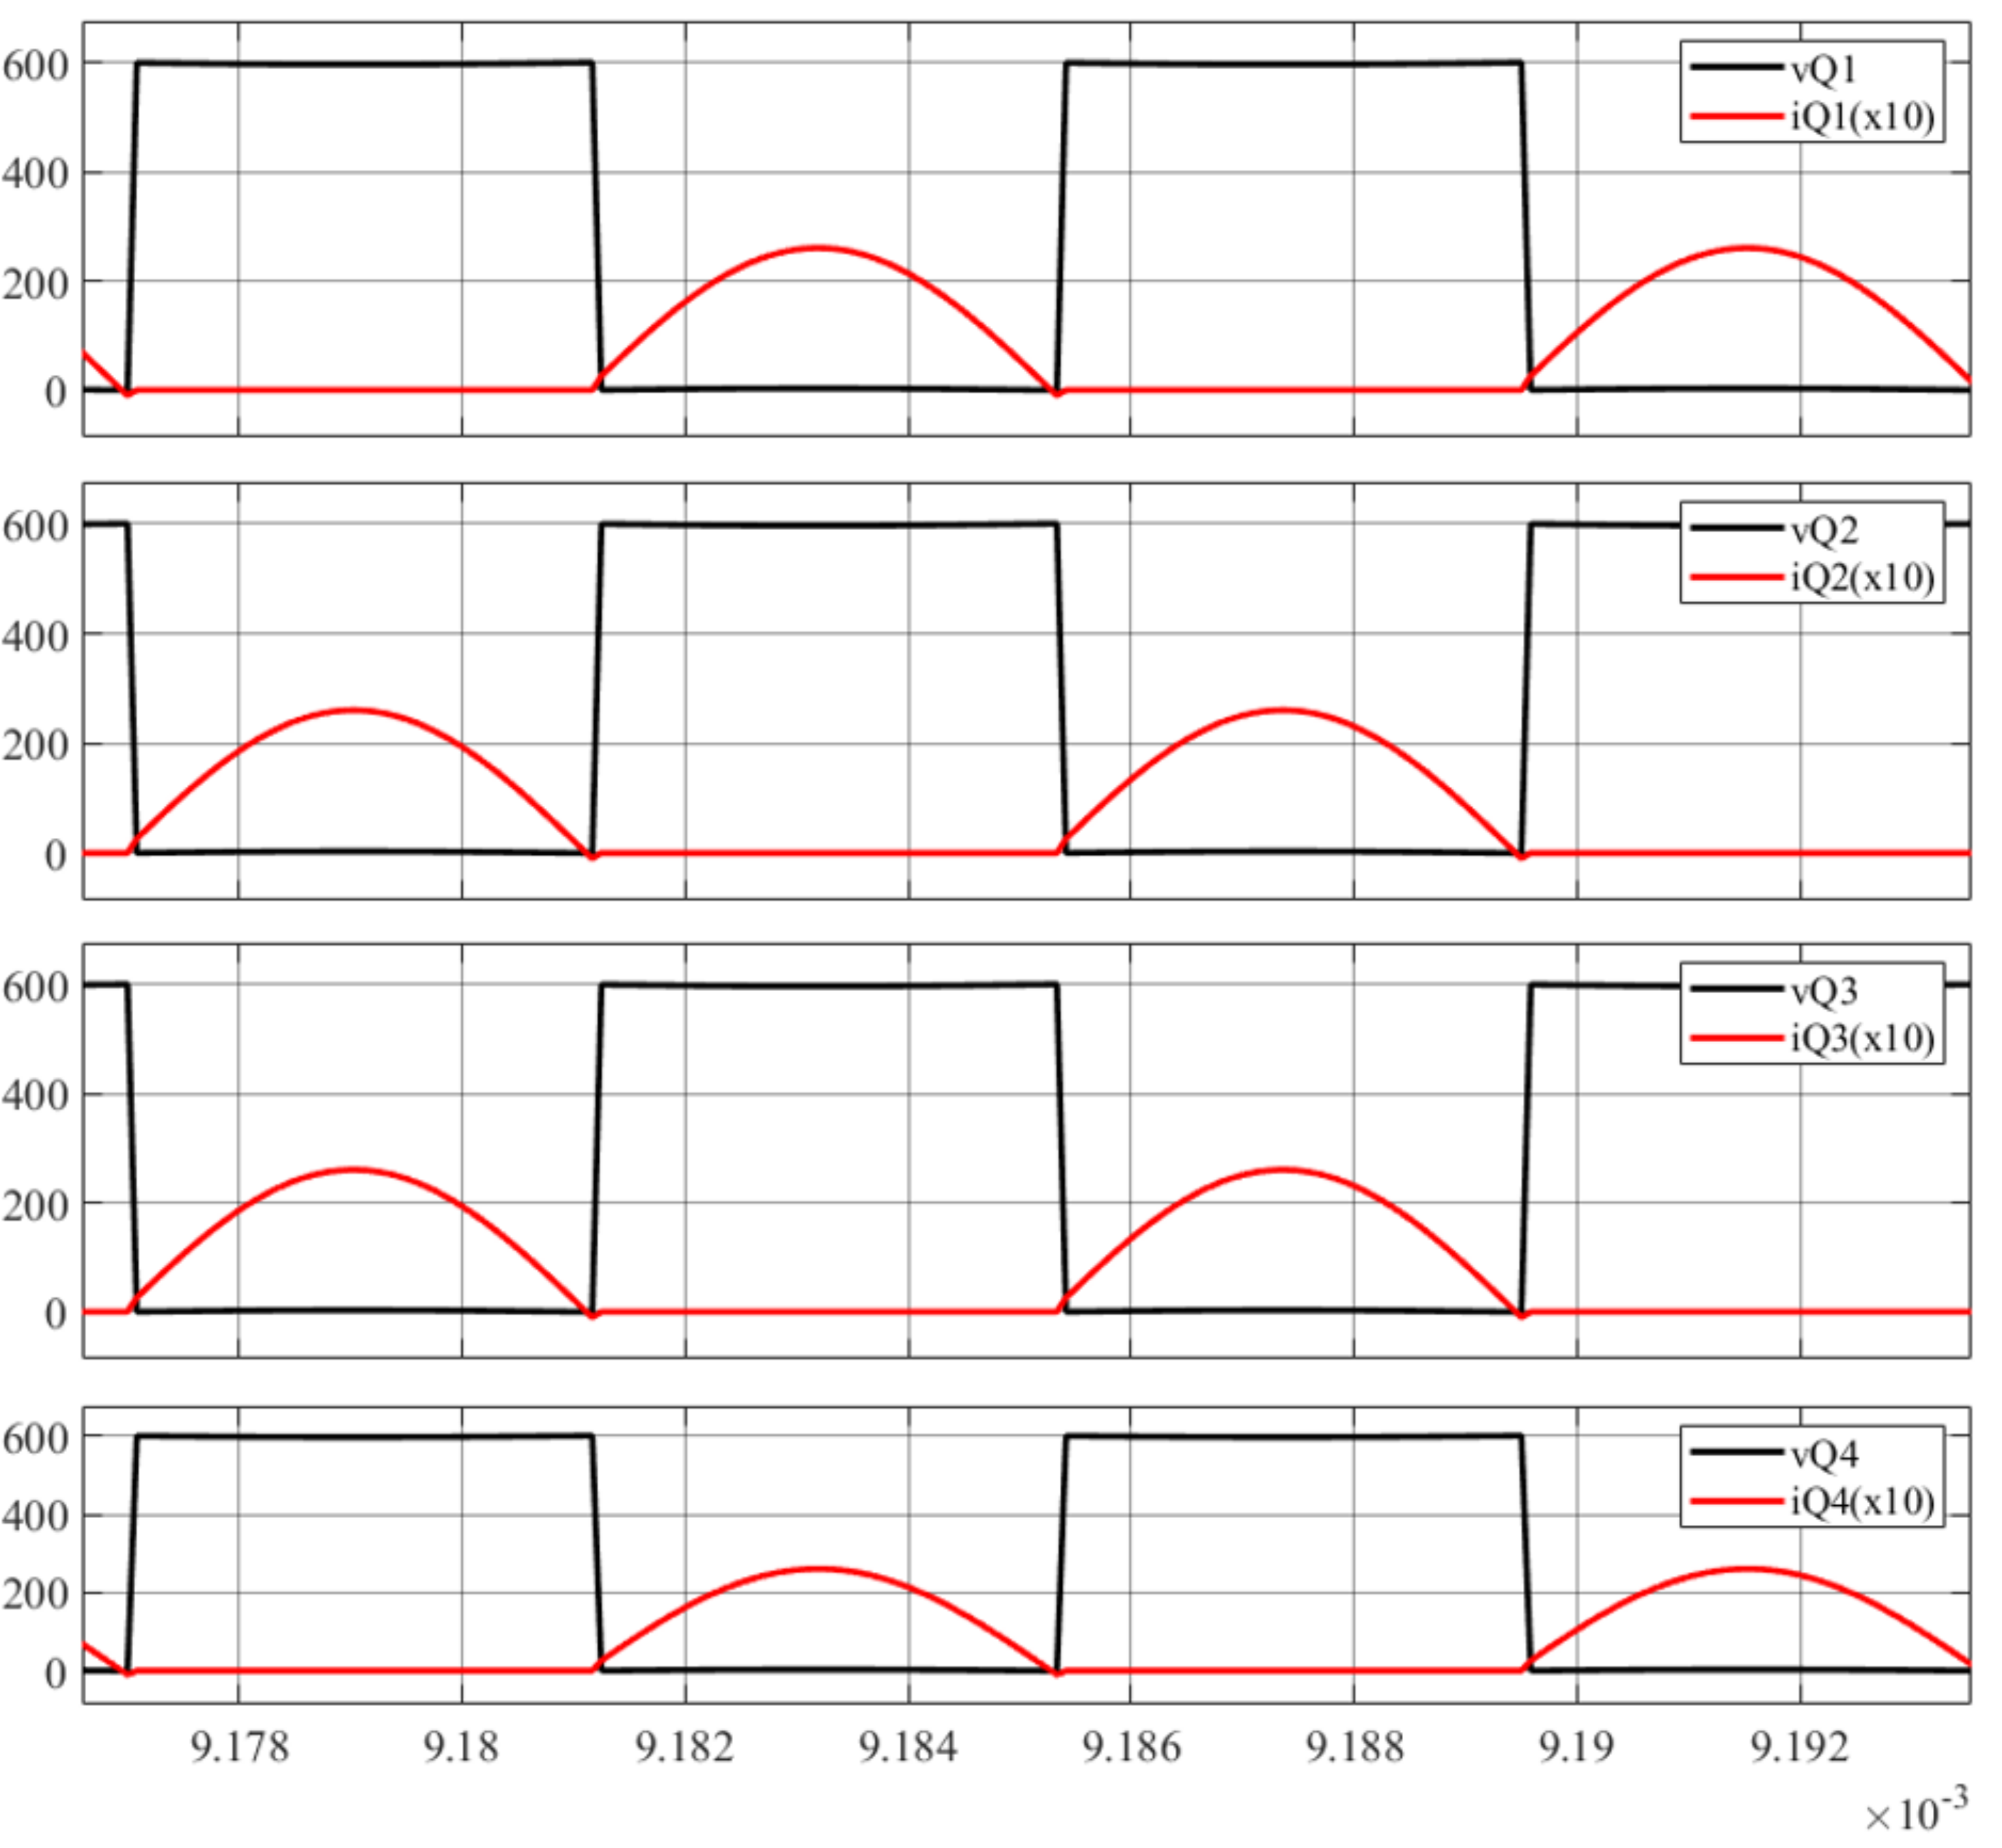
\includegraphics[width=.95\columnwidth]{figures/Result_3.png}
    \caption{Switch voltage and current waveforms.}
    \label{fig:Result_3}
\end{figure}


Fig.~\ref{fig:Result_3} shows the voltage and current waveforms of the switches ($Q_1$--$Q_4$) under steady-state operation at the optimized operating point obtained using the proposed framework. It can be observed that the current through each switch approaches zero prior to commutation, indicating soft-switching conditions with reduced overlap between voltage and current waveforms.

To further demonstrate the effectiveness of the proposed optimization procedure, the optimized operating condition was compared with a non-optimal design operating farther from resonance. The optimized solution exhibited improved soft-switching behavior, reduced switching stress, and higher efficiency, confirming that the proposed framework is capable of identifying operating points associated with enhanced converter performance.

\begin{figure}[!htb]
    \centering
    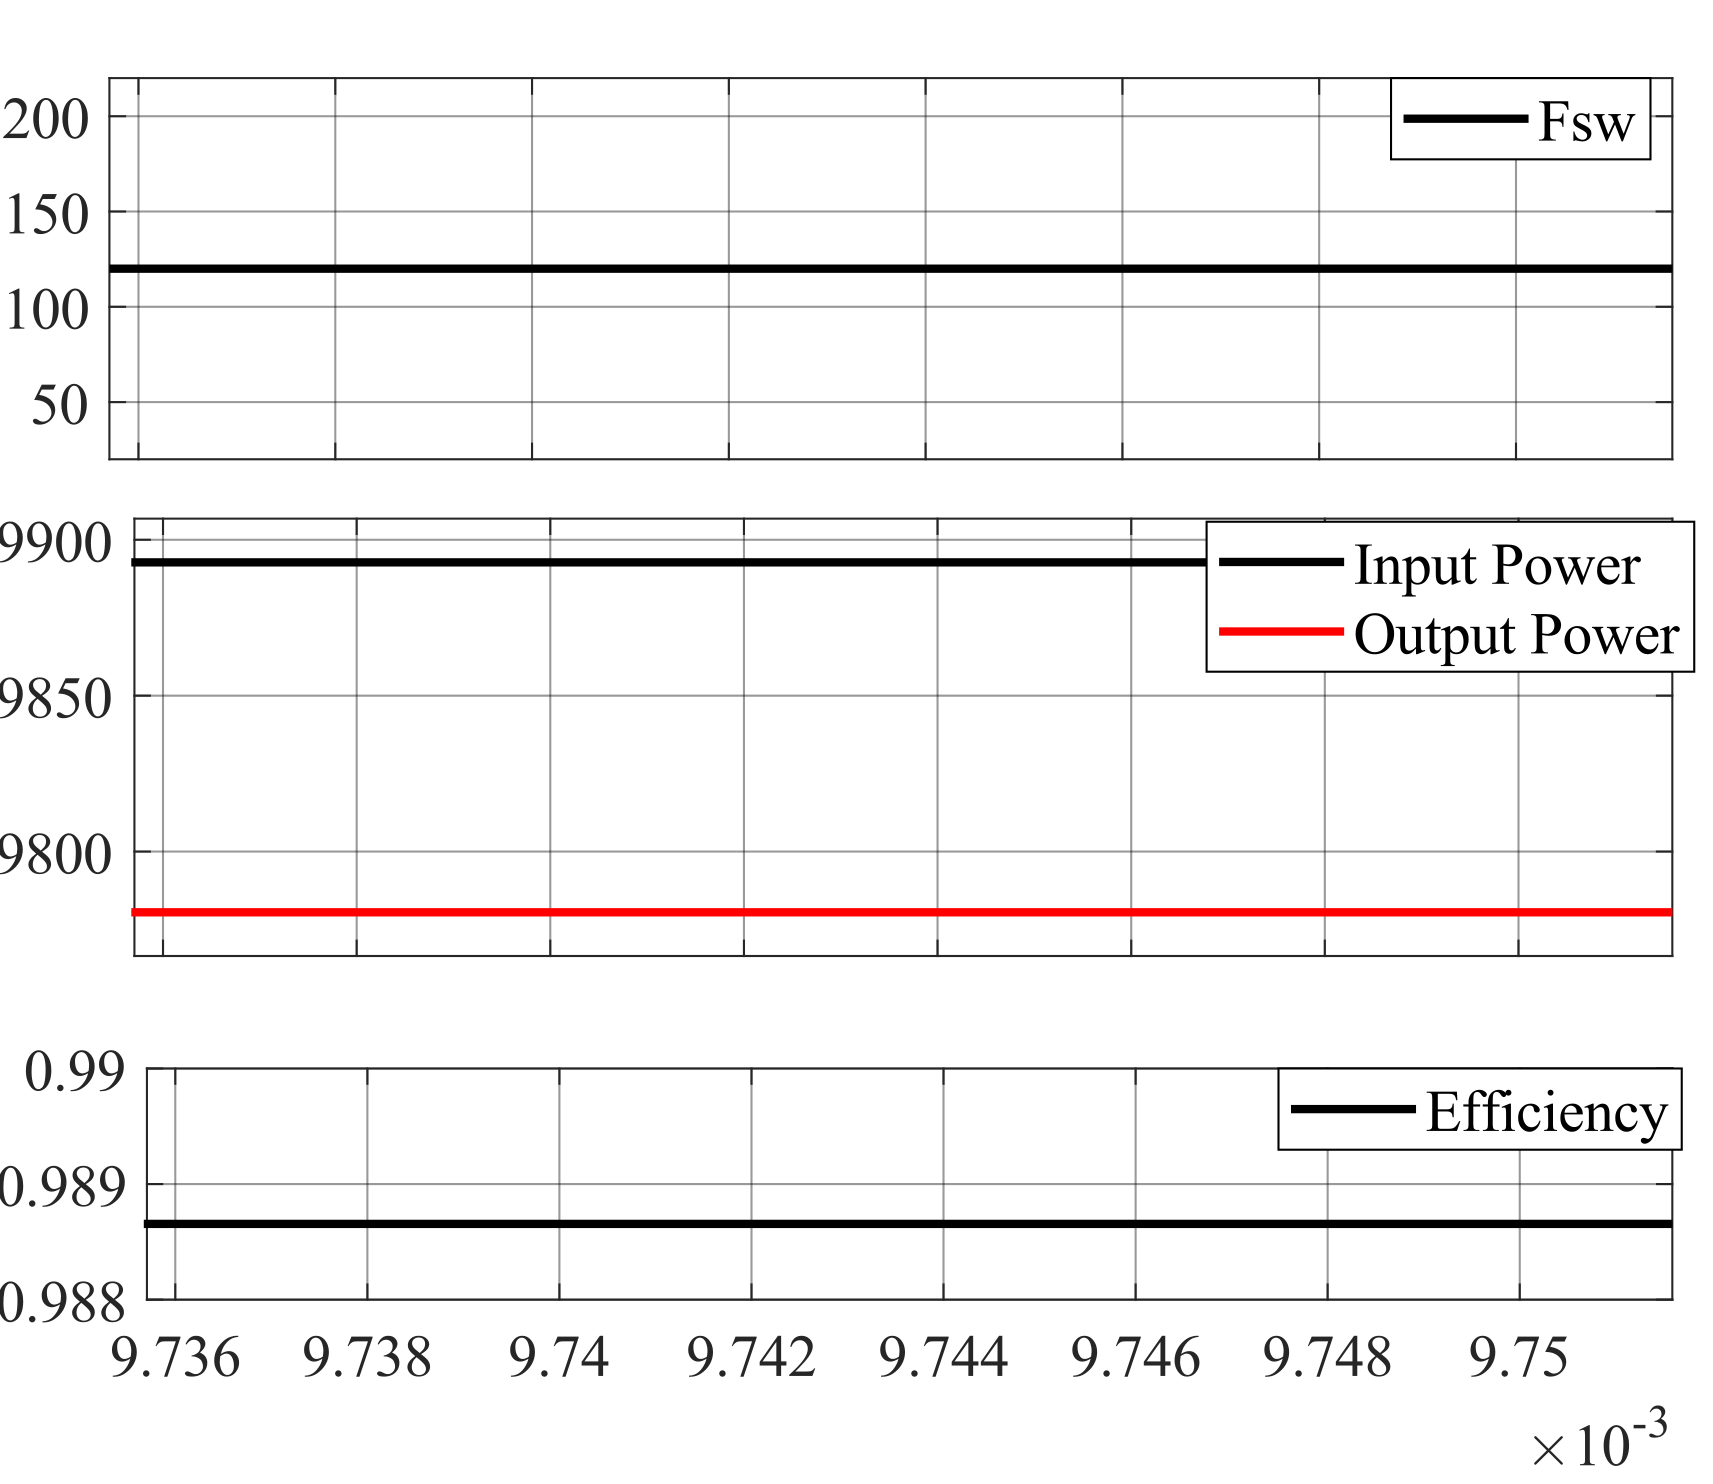
\includegraphics[width=.95\columnwidth]{figures/Result_5.png}
    \caption{Switching frequency, power, and efficiency.}
    \label{fig:Result_5}
\end{figure}

Fig.~\ref{fig:Result_5} shows the switching frequency, input and output power, and the resulting efficiency under steady-state operation. The switching frequency remains constant, indicating stable control. The input and output power levels are also nearly constant, with a small difference corresponding to system losses.

The efficiency remains stable around 98.9\%, indicating high-efficiency operation with limited power dissipation. The consistency of these quantities over time confirms both steady-state behavior and the reliability of the efficiency calculation.

